\section{Implementation}
\label{sec:implementation}

The Bitcoin Blockchain for the period of 2009 until March of 2017 constitutes
from blocks with a total size of approximately 98GBs. We analyze the data using
Apache Spark~\cite{Zaharia} with Scala and an open-source tool that integrates
very well with Spark, HadoopCryptoledger~\cite{cryptoledger}. HadoopCryptoLedger 
provides us with the ability to form the block and transaction objects as well as 
an example on how to construct the transactions graph. Since we have to do graph-processing
to compute our metrics we need a tool that cooperates impeccable with Apache
Spark in parallel and distributed computing; thus, the use of
GraphX~\cite{graphx} is decisive. After computing the metrics, we create
interactive visualizations of the results into a Bootstrap~\cite{bootstrap}
HTML website using Chart.js~\cite{chartjs}. We use \textit{Bar Charts} to represent the years, \textit{Line Charts} for the months of each yearand one \textit{Pie Chart} for the Size that demostrantes the contributed percentage of 
each year to the total of the graph. For the visualization of the
community that provides the Conductance of the graph, we use gexf-js.js~\cite{gexfjs}
which cooperates well with Gephi~\cite{gephi} and allows us to visualize the results into the website. 
We store all the data of the Bitcoin Blockchain into HDFS and we compute the metrics on a small part of the Dutch
national e-infrastructure with the support of SURF Cooperative.

\begin{figure*}[h!]
	\centering
	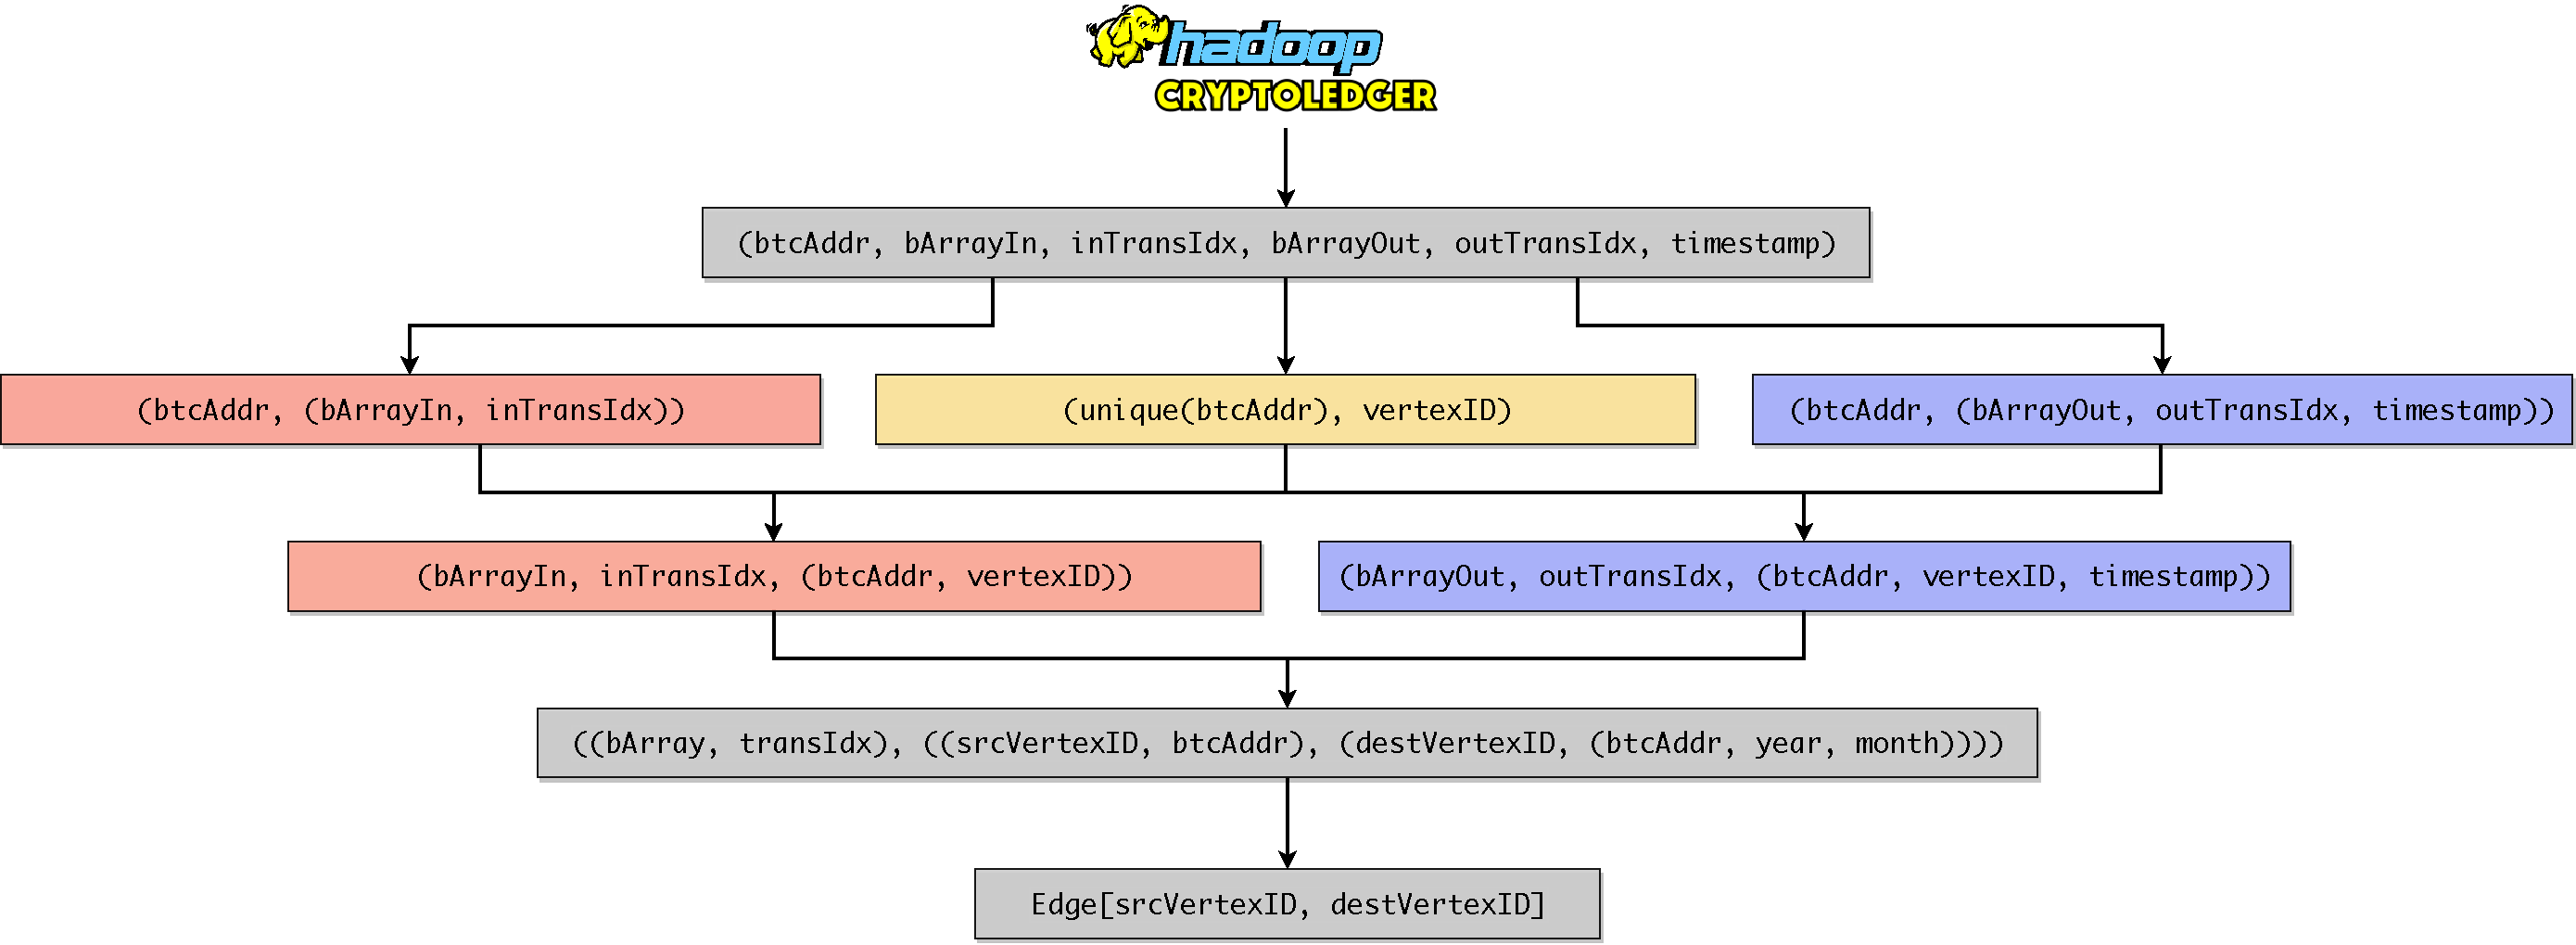
\includegraphics[width=1\linewidth]{./images/fig2}
	\caption{The steps of producing the edges of the graph. We construct the graph only from the edges and we only the source and destination vertex ID from the final results of the process. Hence, we keep those as well as the timestamp which we convert to date in order to partition the graph to different timesnapshots.}
	\label{fig:fig2}
\end{figure*}

\subsection{Transactions Graph}
The foundations of this work is the great size of our data and how we treat them. Our dataset consists of 98GBs of Bitcoin Blockchain blocks. Since the amount of data is big enough to use them for the metrics computation without any pre-processing, we filter out everything that we do not need. As we describe in~\secref{sec:background} each block in the Blockchain contains numerous information, but for the purposes of our analysis we only need the timestamp and the transactions list. Our approach to represent the graph, is that every Bitcoin address is a vertex and every transaction is a directed edge from one vertex to another.

Each transaction in the list is constructed from input and output transactions,
where the input transactions come from previous blocks. HadoopCryptoledger
deserializes the blocks and iterates through each transaction entry in the list
and returns the \textit{destination Bitcoin address}, the \textit{input} and \textit{output ByteArray} and the \textit{index of the input} and 
\textit{output transaction} in the list. However, the timestamp of the block is missing. Thus, we modify the
code and we add it to the returning results. 

Since the Bitcoin addresses represent the vertices in a graph, we gather all
the unique addresses, we store them into an RDD and we assign them a vertex ID.
To construct the edges, we need to join all the input with the output
transactions. First, we construct the input and output transactions RDDs and we assign the timestamp
only to the output transaction to avoid confusion of the dates coming from
previous blocks after the join. For instance, if we assign the timestamp to
both, we can end up with the input transaction date being later than the
output, which is impossible since the input transactions come from previous
mined blocks.

Before joining the input and output RDDs to obtain the edges, we first need the
vertex ID on each row of both RDDs since it will represent the source and
destination of our edge. Hence, we join each RDD with the one that contains the
unique Bitcoin addresses. We then join the results on
the ByteArray and the transaction index and we end up with the edges for the
graph. However, we do not need neither all the information of the results nor
the vertices, since we can construct the graph only from the edges. Thus, we
discard everything and we keep only the timestamp and the source and
destination vertex ID. Finally, we convert the final RDD into a DataFrame in
order to convert the timestamp to date and partition the graph on certain time
snapshots. We keep only the year and month columns and we partition the edges
by them storing the results into HDFS as parquet files. Each time, not only we
are able to load the graph for the desired timesnapshot but also we manage to
reduce the size of the data from 98GBs to 14GBs.~\fref{fig:fig2} demonstrates
the procedure described above.


\subsection{Metrics Implementation}

Based on the formulas described in \secref{sec:background} we implement our
algorithms in Scala by the agency of GraphX which provides several functions
for graph-processing~\cite{graphxDoc}. The metrics that we compute are mostly
iterative algorithms that need a lot of time as the size of the graph increases each year. 
Below we describe the methodology that we follow in order to
compute each metric, as well as some functions of GraphX that proved to be really handy.

\subsubsection{Size}
Computing the Size of a graph is simple process as we just need to count the total number of edges. We use the function \textit{Graph.numEdges} that GraphX provides.

\subsubsection{Triangle Participation Ratio}
For the Triangle Participation Ratio the proccess we follow is to find the total number of vertices that participate in a triangle. For this step we use the function \textit{Graph.triangleCount} of GraphX, we filter out the vertices that do not participate in any triangle and then, we divide the result with the total number of vertices of the graph.

\subsubsection{Bridge Ratio} Our approach to compute Bridge Ratio is to use the
DFS traversal algorithm with a complexity of O(V\texttt{+}E). The main idea is
to keep track of the visited vertices by finding the neighbors of each vertex,
go through them, and store parent vertices in a DFS tree. In order to find the
neighbors of each vertex we use the \textit{Graph.collectNeighborIds} function from
GraphX. Then, we check if the subtree rooted with the current neighbor of the
vertex has a connection to one of the ancestors of the specific vertex. If the
lowest vertex reachable from the subtree under the specific vertex is below its
parent vertex in the DFS tree, then the edge that connects the current 
and its parent vertex is a bridge.

\subsubsection{Global Clustering Coefficient}
For the Global Clustering Coefficient, the urgent matter is to compute the total number of triangles as well as the total number of open and close triplets. For that reason, we use the functions \textit{Graph.trianglesCount} and \textit{Graph.triplets} of GraphX, to compute respectively each of the above. Then, we multiply with 3 the number of triangles and divide them by the total number of triplets.

\subsubsection{Conductance}
To compute Conductance, we first need to generate the K non-overlapping cuts. For that reason we apply the \textit{Label Propagation} algorithm in order to split the graph into communities. We perform 10 iterations and then we discard the communities containing less than 10 edges since their importance compared to the size of other communities has minor importance for the result. As we further analyze in~\secref{sec:discussion}, due to the complexity of the computation, we choose only the top 10 communities in edgs for the computation. For those communities we compute the fraction of edges going out to the minimun total edges and we report the minimum of those values.

\subsubsection{Average Clustering Coefficient \& Diameter}
In order to compute the Average Clustering Coefficient, we use the implementation of Sherlock Yang~\cite{localCCgit}, that computes the Local Clustering Coefficient for each vertex. The Average Clustering Coefficient derives from summing the results and finding the mean value. In addition, the Diameter implementation is equivalent with the one derivered from~\cite{diam1, diam2} and can be found on publicly available at GitHub~\cite{diamGit}.

